% !TEX root = ../Bachelorthesis.tex
%
%************************************************
% Einführung
%************************************************
\chapter{Einführung}
\label{sec:Einfuehrung}

Springer Nature ist ein weltweit führender Verlag für Forschungs-, Bildungs- und Fachliteratur mit einer breiten Palette an angesehenen und bekannten Medienmarken und zudem der weltweit größte Verlag für Wissenschaftsbücher. Für das Unternehmen Springer Nature ist es darum wichtig, auf seinen Web-Applikationen eine Suche anbieten zu können, die Suchintentionen erkennt und möglichst schnell zum gesuchten Content leitet. Die Suche wird vor allem als Hilfsmittel zur Navigation und zum Finden von Literatur und Dienstleistungen genutzt. Durch die vielen von Springer Nature publizierten Zeitschriften und Querverweise in Artikeln, wird sie aber auch oft zur Suche nach Issues\footnote{Nummer der Zeitschriftenausgabe, in der sich der Artikel befindet.} und Artikeln verwendet sowie als Hilfestellung um Diagnosen zu Krankheitsbilder stellen zu können.
\\
\\
Springer Nature sammelt viele User-Tracking-Daten und dadurch viel Wissen über das Verhalten der User\footnote{Als User werden die Nutzer der Springermedizin-Suche bezeichnet} bei der Nutzung ihrer Suche, lässt dieses Wissen jedoch bisher noch nicht in ihre Suche einfließen. In dieser Arbeit wollen wir untersuchen, ob mithilfe dieses Wissens, die Suche optimiert werden kann.

\section{Aufbau der Suche bei Springer Nature}
\label{sec:Einfuehrung:AufbauSucheBeiSpringerNature}

\subsubsection{White Label Applikation mit Solr-Suche}
\label{sec:Einfuehrung:AufbauSucheBeiSpringerNature:WhiteLabelApplikationSolr-Suche}

Damit die verschiedenen Verlage und Zeitschriften der Verlagsgruppe Springer Nature ihre Produkte und Dienstleistungen online anbieten können nutzt Springer Nature eine eigens entwickelte White Label Applikation\footnote{Eine White Label Applikation ist eine wiederverwendbare und agil erweiterbare Applikation}. Die White Label Applikation verwendet \textit{Apache Solr} (im Folgenden "Solr" genannt)~(siehe \cite{solr}) als Suchplattform. Die Solr dient hierbei als eine der Schnittstellen zwischen dem Content-Pool von Springer Nature und der White Label Applikation. Bei den vom Content-Pool gelieferten Inhalten, handelt es sich um von Springer Nature Verlag publizierte Zeitschriften, Artikel, Bücher und redaktionelle Inhalte.

\subsubsection{User-Tracking mit Webtrekk}
\label{sec:Einfuehrung:AufbauSucheBeiSpringerNature:Webtrekk}

Um das Verhalten der User auf ihren Web-Applikationen zu tracken verwendet Springer Nature das Analysetool Webtrekk~(siehe \cite{webtrekk}). Die daraus resultierenden Berichte bieten unter anderem die Möglichkeit, \textit{Suchquery-Logs}\footnote{Protokoll über alle ausgeführten Suchanfragen auf der Applikation} und \textit{Click-Trough-Rates} (CTR)\footnote{Kennzahl um die Anzahl der Klicks auf Links im Verhältnis zu den gesamten Impressionen darzustellen} der User auszuwerten.

\pagebreak

\subsubsection{Architektur}
\label{sec:Einfuehrung:AufbauSucheBeiSpringerNature:Architektur}

In Abb. \ref{fig:SucheSpringerNature} ist die Suche nochmals grafisch aufbereitet:

\begin{figure}[H]
\centering
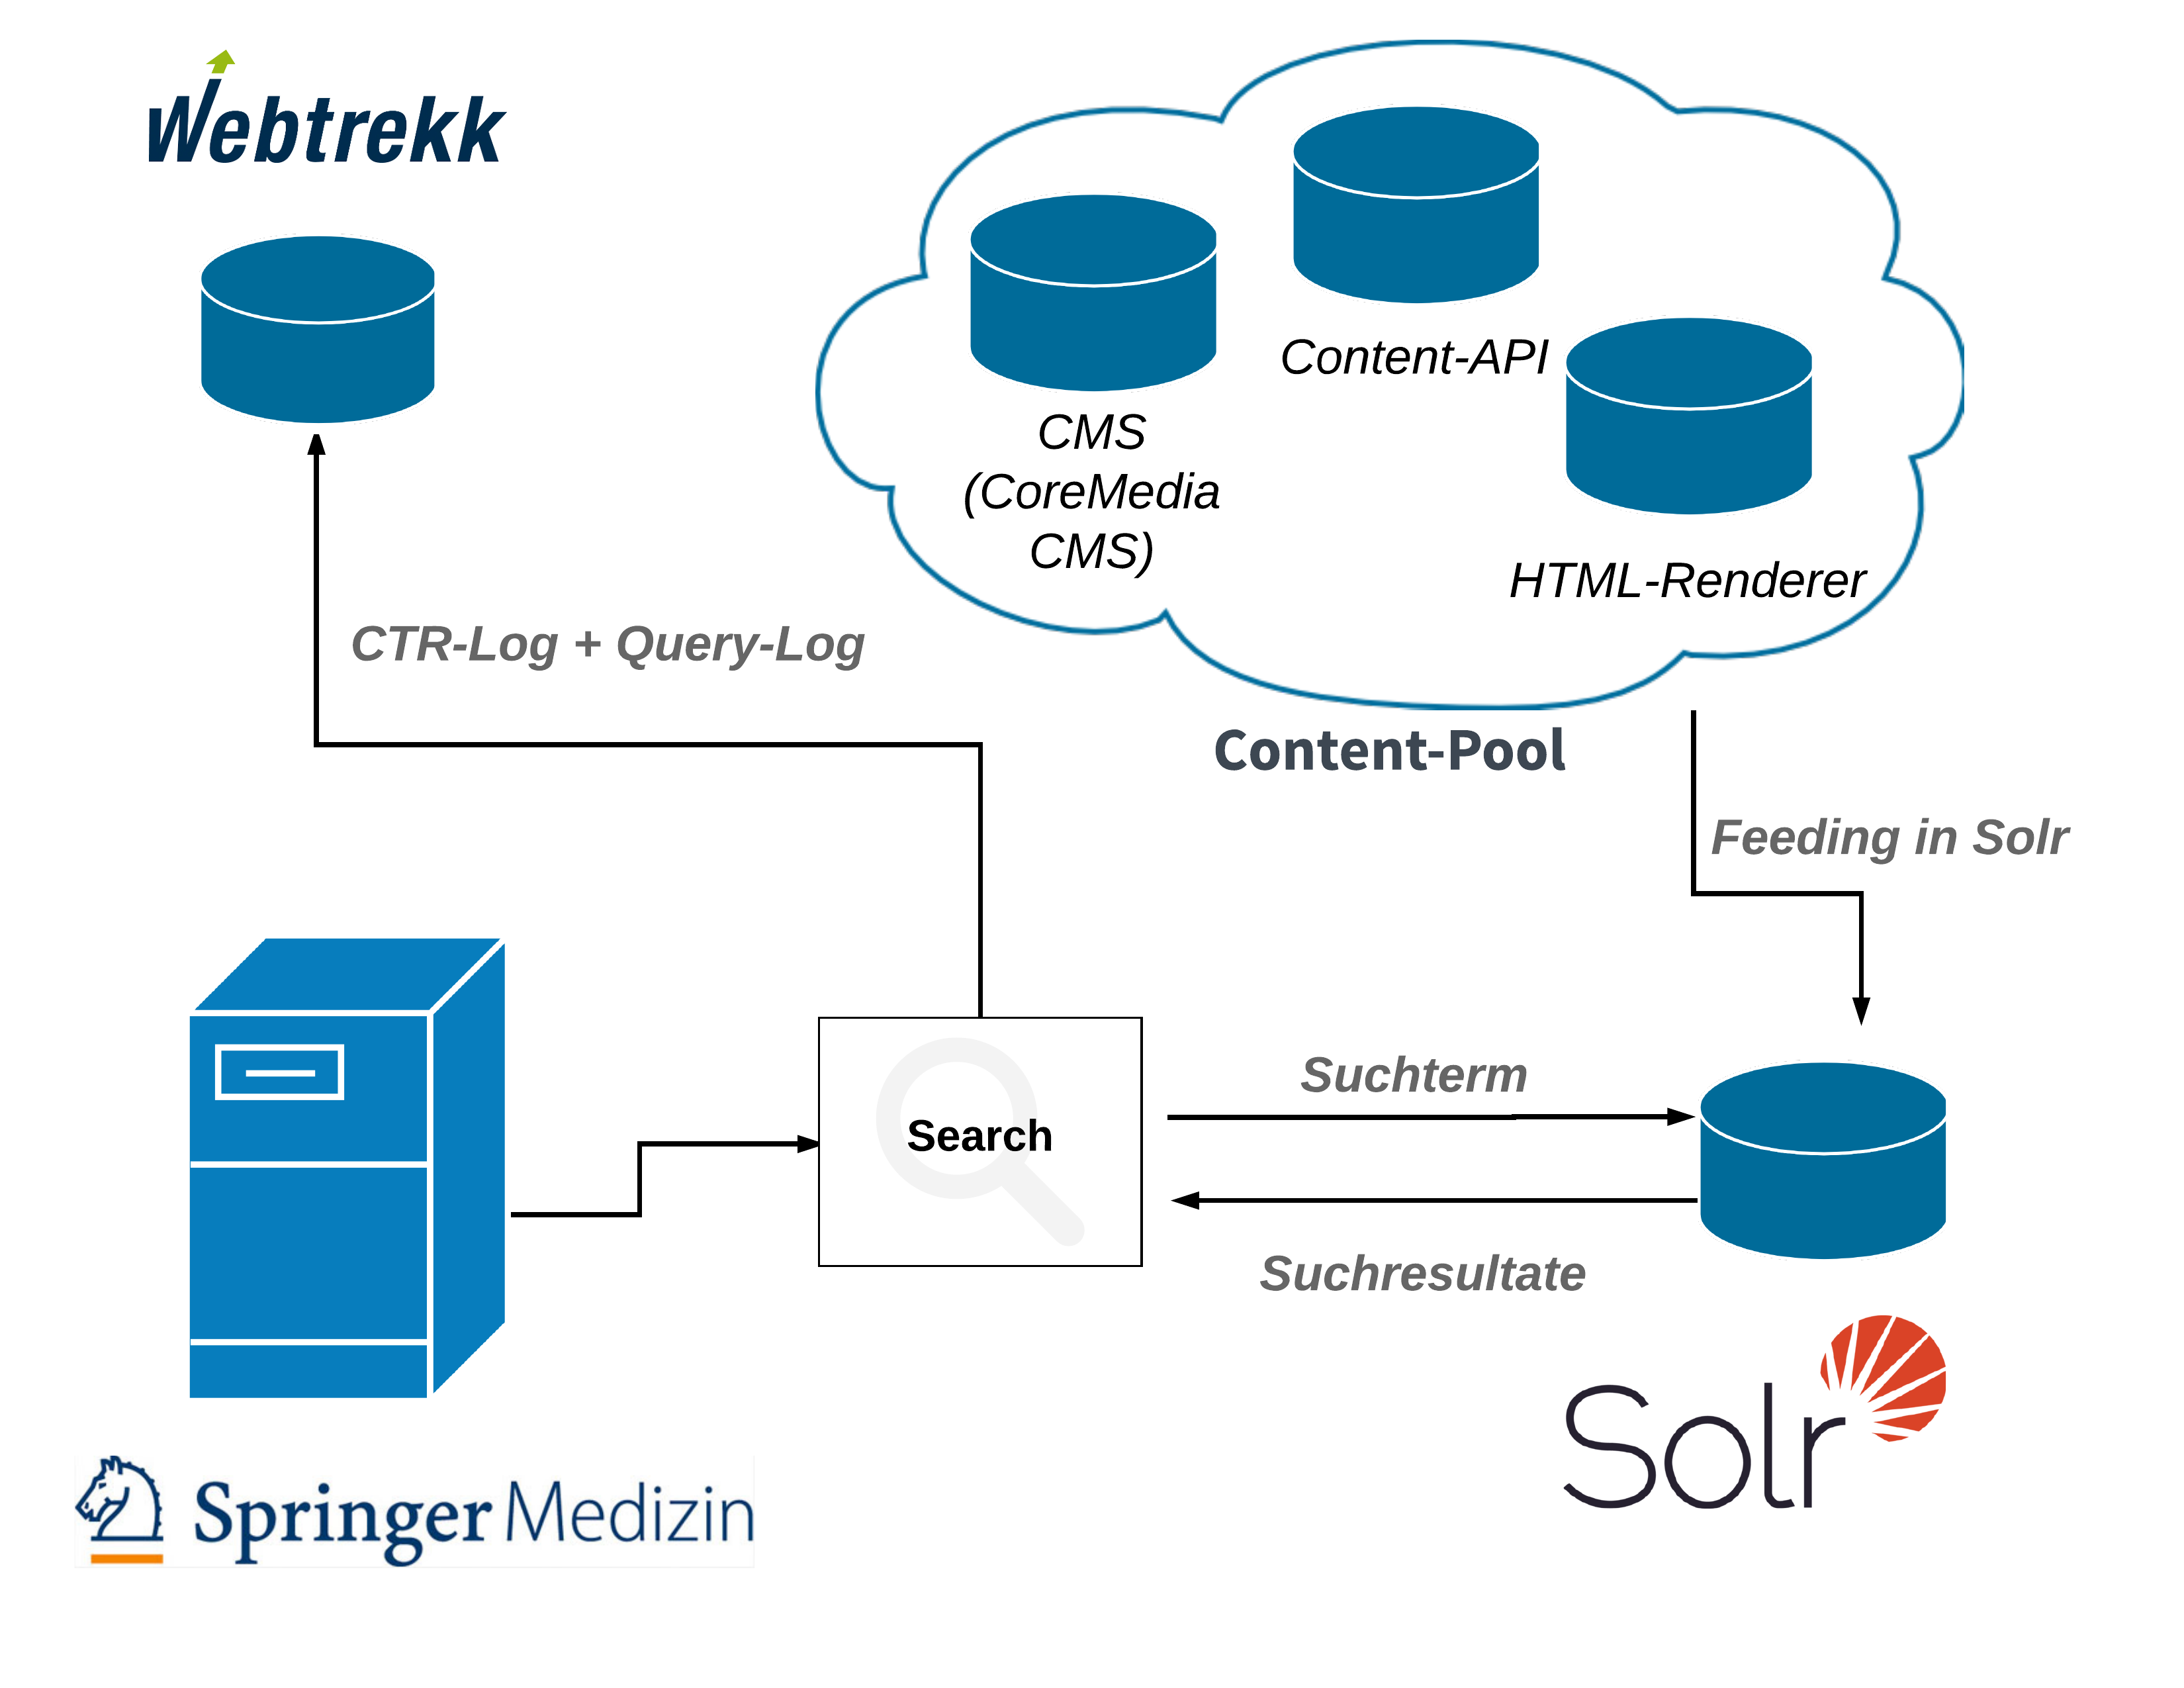
\includegraphics[width=0.5\linewidth]{gfx/AufbauSucheSpringerNature}
\caption[Aufbau der Suche bei Springer Nature]{Aufbau der Suche bei Springer Nature}
\label{fig:SucheSpringerNature}
\end{figure}

\section{Problemstellung: Keine Userrelevanz in der Suche}
\label{sec:Einfuehrung:Problemstellung}

\subsubsection{Userrelevante Dokumente werden nicht gefunden}
\label{sec:Einfuehrung:Problemstellung:Userrelevanz}

Die User von Springermedizin suchen oft mit einschlägig, fundierten Fachbegriffen nach den neuesten und relevantesten Zeitschriften, Bücher oder Publikationen. Die zeitlich aktuellsten Suchtreffer zu finden ist für Springermedizin kein Problem. Die für den User \textit{relevantesten} jedoch schon.

\subsubsection{Der Springer Nature Stakeholder: Springermedizin setzt auf Webtrekk}
\label{sec:Einfuehrung:Problemstellung:Springermedizin}

Zu den Stakeholder\footnote{Bezeichnet Springer Nature interne Kunden, die ein Interesse am Ergebnis der White Label Applikation haben} der in Kapitel \ref{sec:Einfuehrung:AufbauSucheBeiSpringerNature:WhiteLabelApplikationSolr-Suche} angesprochenen White Label Applikation gehört \textit{Springermedizin}~(siehe \cite{SMED}). Springermedizin ist ein Fortbildungs- und Informationsportal für Ärzte. Mithilfe von Webanalysten und Webtrekk versucht Springermedizin das Marketing seines Webauftrittes zu verbessern und ist sehr interessiert an neuen Ansätzen, um die gesammelten Tracking-Daten besser einzusetzen. In dieser Arbeit wird darum der Fokus auf die Verwendung von Tracking-Daten in der Suche von Springermedizin gesetzt. 
 

\subsubsection{Der fast gläserne User}
\label{sec:Einfuehrung:Problemstellung:Glaeserne-User}

Springermedizin sammelt Tracking-Daten über jegliche Aktivitäten auf deren Applikationen und investiert Zeit und Geld in die Individualisierung\footnote{Mit Individualisierung wird die Speicherung eigener Parameter bezeichnet} der Analysedaten auf Webtrekk. Mittlerweile sind knapp 30 Custom-Parameter\footnote{Individuell erzeugte Parameter für Berichte und Analysen} auf Webtrekk angelegt um genau die Daten zu tracken, die zur Analyse des Verhaltens der User auf ihrer Applikationen relevant sind. Dadurch entsteht ein fast \glqq gläsernen User\grqq{}. Dieses Wissen könnte zum Vorteil des Users eingesetzt werden, indem es in der Suche verwendet wird.

\section{Ziel der Arbeit}
\label{sec:Einfuehrung:ZielArbeit}

\subsection{Suchoptimierung durch Click-Trough-Daten}
\label{sec:Einfuehrung:ZielArbeit:Suchoptimierung}

In dieser Arbeit werden wir untersuchen, ob mithilfe der von Springermedizin gesammelten Click-Trough-Daten dessen Suche verbessert werden kann. Im Idealfall widerspiegeln die gesammelten Click-Trough-Daten der Suchresultate die Userrelevanz der einzelnen Dokumente\footnote{Als Dokumente werden die einzelnen Suchresultate bezeichnet}.

\subsubsection{Annahmen}
\label{sec:Einfuehrung:ZielArbeit:Suchoptimierung:Annahmen}

Wir gehen dabei von folgenden Annahmen aus. Relevante Dokumente sind wichtiger als nicht relevante Dokumente. Eine Suchergebnis ist dann gut, wenn die relevanten Ergebnisse in der verwendeten Hierarchie vor den nicht relevanten Ergebnisse auftauchen. 

\subsection{Abbildung auf das Springermedizin-Umfeld}
\label{sec:Einfuehrung:ZielArbeit:AbbildungSpringermedizinUmfeld}

\subsubsection{Potential von Userrelevanzen in der Suchoptimierung analysieren}
\label{sec:Einfuehrung:ZielArbeit:Potential}

Die Analyse von User-Tracking-Daten bietet viel Potential bezogen auf Userrelevanzen. Sind anhand des hier umgesetzten Lösungsansatzes Verbesserungen in der Qualität der Suche zu verzeichnen, möchte Springermedizin in Zukunft vermehrt User-Tracking-Daten in die Suche einfließen lassen. Diese Arbeit könnte dann als Fundament für weitere Lösungsansätze dienen.

\subsubsection{Bekanntes und wirkungsvolles Information Retrieval Verfahren}
\label{sec:Einfuehrung:ZielArbeit:AbbildungSpringermedizinUmfeld:InformationRetrievalVerfahren}

Suchoptimierung mittels Userrelevanz ist ein bekanntes und nicht triviales, aber relativ wirkungsvolles Information Retrieval Verfahren~(siehe \cite{IWUSBI}). Seit Mitte der 2000er Jahre wird mithilfe dieses Verfahrens versucht, Suchmaschinen zu verbessern. Aus dieser Zeit stammen auch die ersten Ansätze um mithilfe von Click-Trough-Daten die Userrelevanz der Suchergebnisse zu berechnen~(siehe \cite{Joachims}).

\subsubsection{Lösungsansatz basierend auf Click-Trough-Daten aus Webtrekk}
\label{sec:Einfuehrung:ZielArbeit:AbbildungSpringermedizinUmfeld:Loesungsansatz}

Springermedizin führt ein eigenes Tracking der User durch und verwendet auf Webtrekk selbst definierte Tracking-Parameter. Dadurch hängt die Wahl des in dieser Arbeit zu untersuchenden Lösungsansatzes und dessen Umsetzung stark von den durch Webtrekk gegeben Analyse-Daten ab.

\subsubsection{Anwendung auf Springermedizin-Umfeld}
\label{sec:Einfuehrung:ZielArbeit:AbbildungSpringermedizinUmfeld:Adaptierung}

Bei der Verwendung von Userrelevanzen in der Suche handelt es sich um ein bekanntes und gut erforschtes Problem. Wir werden in dieser Arbeit versuchen, einen bestehenden Lösungsansatz (Position-based Modell) auf das Springermedizin-Umfeld abzubilden. Die Herausforderung wird hierbei die Adaptierung des Lösungsansatzes auf das Springermedizin-Umfeld sein.

\subsubsection{Was wird in dieser Arbeit nicht behandelt?}
\label{sec:Einfuehrung:ZielArbeit:AbbildungSpringermedizinUmfeld:NichtBehandeln}

Durch den vorgegebenen Zeitraum für die Erstellung dieser Bachelorarbeit bedingt, werden wir den Lösungsansatz so wählen, dass er mit den Gegebenheiten bei Springermedizin sinnvoll und in diesem Zeitrahmen realistisch implementiert werden kann. Wir werden daher in dieser Arbeit keine Gegenüberstellung mit anderen Lösungsansätzen machen. 
\\
\\
Bei der Umsetzung des Lösungsansatzes konzentrieren wir uns auf die Implementation des Algorithmus zur Berechnung der Userrelevanz. Die semantische Aufschlüsselung von Suchtermen ist nicht Kern dieser Arbeit. Die semantische Aufschlüsselung des Suchterms\footnote{Als Suchterm wird eine Suchanfragen bezeichnet} zur Analyse der Webtrekk-Daten enthält darum keine Gewichtungen der Relationen zwischen Webtrekk-Daten und Suchterm. Alle Relationen werden gleich gewichtet. 

\section{Methodik}
\label{sec:Einfuehrung:Methodik}

\subsection{Einführung}
\label{sec:Einfuehrung:Methodik:Einfuehrung}

Wie in Kapitel \ref{sec:Einfuehrung:ZielArbeit:Suchoptimierung} angesprochen, wollen wir das Klick-Verhalten der User in der Suche analysieren um mithilfe der daraus berechenbaren Userrelevanzen die Suchergebnisse zu verbessern. Dieses Klick-Verhalten können wir aus den Click-Trough-Daten lesen. Um mit Click-Trough-Daten arbeiten zu können, müssen wir zuerst verstehen, was Click-Trough-Daten sind und wie sie entstehen. 

\subsection{Click-Trough-Daten verstehen}
\label{sec:Einfuehrung:Methodik:Click-Trough-Daten}

\subsubsection{Was sind Click-Trough-Daten und wie entstehen diese?}
\label{sec:Einfuehrung:Methodik:Click-Trough-Daten:WasSindClick-Trough-Daten}

Click-Trough-Daten sind Tracking-Daten. Tracking-Daten entstehen durch die Interaktion zwischen dem User der Applikation und der Applikation selbst. Sie verfolgen das Verhalten der User auf der Applikation und speichern diese in einer Datenbank, in unserem Fall in Webtrekk ab. Die für uns interessanten Tracking-Daten entstehen, wenn der User auf der Suche von Springermedizin ein Anfrage stellt und darauf folgend, ein Element aus dem Suchresultat anklickt.

\subsubsection{Wie werden die Click-Trough-Daten in Webtrekk gespeichert?}
\label{sec:Einfuehrung:Methodik:Click-Trough-Daten:SpeichernClick-Trough-Daten}

Die Speicherung der Daten auf Webtrekk übernimmt die Springermedizin-Applikation. Führt ein User eine Suche durch und klickt dabei ein Resultat an, sendet die Springermedizin-Applikation die Tracking-Informationen an Webtrekk. Die Tracking-Daten für diese Aktion, setzen sich zusammen aus der Suchanfrage, dem Zeitpunkt der Suche, den Userdaten, der angeklickten Position im Suchresultat und den Dokumentinformationen zum angeklickten Dokument. Aus diesen Daten werden die Click-Trough-Daten erstellt, mithilfe denen wir die Userrelevanz berechnen werden.

\subsubsection{Wie können wir Click-Trough-Daten aus Webtrekk lesen?}
\label{sec:Einfuehrung:Methodik:Click-Trough-Daten:LesenClick-Trough-Daten}

Webtrekk ist ein Analysetool. Das heißt für uns, wir können nicht direkt auf die Datenbank mit den Tracking-Daten zugreifen. Um die Tracking-Daten lesen zu können, müssen wir eine Analyse auf Webtrekk ausführen. Mithilfe dieser Analyse können wir uns die Click-Trough-Daten so zusammenstellen lassen, wie wir sie für die Berechnung der Userrelevanz benötigen.
\\
\\
Die Click-Trough-Daten bestehen aus einzelnen Click-Trough-Rates. Eine Click-Trough-Rate zeigt die Anzahl der Klicks, die zu einer bestimmten Suchanfrage auf ein bestimmtes Dokument gemacht wurden und auf welcher Position im Suchresultat sich dieses Dokument dabei befunden hat. Die Webtrekk-Analysen geben uns eine Sammlung von Click-Trough-Rates zurück. Wir können bei diesen Analysen die Click-Trough-Rates nach Suchbegriffen oder auch Suchtermen filtern und den Zeitraum mitgeben, in welchen die Suchanfragen durchgeführt wurden. Des weiteren gibt es die Möglichkeit weitere Filter wie die Anzahl zurückzugebender Click-Trough-Rates oder auch den \glqq Login-Status\footnote{Mit Login-Status wird zwischen einem zum Zeitpunkt der Suche auf der Springermedizin-Applikation angemeldeten und nicht angemeldeten User unterschieden} des Users\grqq{} zu setzen. 

\subsubsection{Wie sehen die Click-Trough-Daten aus?}
\label{sec:Einfuehrung:Methodik:Click-Trough-Daten:AussehenClick-Trough-Daten}

Eine Beispiel für eine Click-Trough-Rate wie sie von einer Webtrekk-Analyse ausgespielt wird, sieht wie folgt aus:

\begin{tabular}{|p{0.8\textwidth}|p{0.15\textwidth}|}\hline
	\textbf{Click-Trough-Rate} & \textbf{Anzahl Klicks} \\ \hline
	searchresult-1.Course.chronische Dyspnoe bei Erwachsenen.10621768.chronische Dyspnoe & 1 \\ \hline
 \end{tabular}

Hier die Aufschlüsselung der Click-Trough-Rate:

\begin{tabular}{|p{0.15\textwidth}|p{0.15\textwidth}|p{0.27\textwidth}|p{0.1\textwidth}|p{0.2\textwidth}|}\hline
	\textbf{Position} & \textbf{Dokumenttyp} & \textbf{Titel} & \textbf{ID} & \textbf{Suchterm} \\ \hline
	searchresult-1 & Course & chronische Dyspnoe bei Erwachsenen & 10621768 & chronische Dyspnoe \\ \hline
 \end{tabular}
 
Die Click-Trough-Rate lässt sich wie folgt lesen. In diesem Beispiel haben die User mit der Suchanfrage \glqq chronische Dyspnoe\footnote{Als Dyspnoe wird eine unangenehm erschwerte Atemtätigkeit bezeichnet}\grqq{} gesucht. Dabei haben sie das Dokument mit der ID 10621768 angeklickt. Dieses hat sich dabei auf der Position 1 der Suchresultate gefunden. Es wurde insgesamt einmal angeklickt in der gesuchten Periode. 

\subsection{Reranking mittels Click-Trough-Rate}
\label{sec:Einfuehrung:Methodik:Reranking}

Im vorherigen Abschnitt haben wir gelernt wie Click-Trough-Daten entstehen und wie sie zu lesen sind. Nun können wir mit diesem Wissen die Userrelevanzen der Dokumente im Suchresultat zur Suchanfrage berechnen. Mithilfe der berechneten Userrelevanzen werden wir dann ein \textit{Reranking}\footnote{Mit Reranking bezeichnen wie die Umsortierung einer Liste von Suchresultaten} der Suchresultate durchführen. So wollen wir die Userrelevanz in die Suche einbinden. Die Vorgehensweise dazu sieht wie folgt aus.

\subsubsection{Suchterm semantisch aufschlüsseln}
\label{sec:Einfuehrung:Methodik:Reranking:SuchtermSegmentierung}

Um die Userrelevanz berechnen zu können müssen wir zunächst die relevanten Click-Trough-Daten filtern. Click-Trough-Daten müssen nicht immer mit dem vollständigen Suchterm in Relation stehen. Sie können auch nur mit einem Wort des Suchterms oder einem Synonym des Wortes in Relation stehen. Wir müssen darum den Suchterm semantisch aufschlüsseln um alle relevanten Click-Trough-Daten filtern zu können. 

\subsubsection{Aufbereitung Click-Trough-Daten}
\label{sec:Einfuehrung:Methodik:Reranking:Click-Trough-Daten}

Können wir alle relevanten Click-Trough-Daten zu einer Suchanfrage filtern, müssen lernen wie wir diese richtig aufbereiten, um die Userelevanzen berechnen zu können. 

\subsubsection{Userrelevanz in Suchprozess einbinden}
\label{sec:Einfuehrung:Methodik:Reranking:SucheEinbinden}


\subsubsection{Result-Reranking mittels PBM Algorithmus}
\label{sec:Einfuehrung:Methodik:Reranking:Result-RerankingPBM}

\subsubsection{Vergessen der alten Daten}
\label{sec:Einfuehrung:Reranking:Vergessen}


\section{Gliederung und Aufbau}
\label{sec:Einfuehrung:GliederungAufbau}

\subsubsection{Der Lösungsansatz und deren Grundlagen}
\label{sec:Einfuehrung:GliederungAufbau:Loesungsansatz}

Im ersten Kapitel wurde der zu untersuchenden Lösungsansatz vorgestellt. Dabei sind wir auf die Hintergründe dieser Arbeit und die Vorgehensweise eingegangen. Im zweiten Kapitel (Grundlagen) folgt die Theorie des beschriebenen Lösungsansatzes. Hier werden wir uns auf die fachlichen Grundlagen konzentrieren. 

\subsubsection{Umsetzung des Lösungsansatzes}
\label{sec:Einfuehrung:GliederungAufbau:Umsetzung}

In Kapitel 3 (Reranking mittels Click-Trough-Rate Ergebnis) werden wir die in Kapitel \ref{sec:Einfuehrung:Methodik} angesprochene Methodik verfeinern und detailliert die Vorgehensweise bei der Umsetzung diskutieren. Die Umsetzung selbst folgt dann in Kapitel 4 (Implementierung).

\subsubsection{Erkenntnisse verarbeiten}
\label{sec:Einfuehrung:GliederungAufbau:Erkenntnisse}

Um zu prüfen ob der umgesetzte Lösungsansatz die erhofften Verbesserungen erzielt, werden wir diesen in Kapitel 5 (Evaluation und Auswertung) in einer Evaluation mit der bisherigen Springermedizin-Suche vergleichen. Aufgrund der resultierenden Erkenntnisse werden wir in Kapitel 6 ein Fazit ziehen können und einen Ausblick auf mögliche zukünftige Arbeiten geben.